\section{Spectral method}
\begin{frame}
	\scriptsize
	Consider 
	\begin{align}
		\textcolor{blue}{\partial_t f}+ \textcolor{gray!80}{\nabla_{\boldsymbol{x}} \cdot(\boldsymbol{u} f)} & +\textcolor{blue}{\nabla_{\boldsymbol{n}} \cdot\left(P_{\boldsymbol{n}^{\perp}} \nabla_{\boldsymbol{x}} \boldsymbol{u} \boldsymbol{n} f\right)}-\textcolor{gray!80}{\nabla_{\boldsymbol{x}} \cdot\left((I+\boldsymbol{n} \otimes \boldsymbol{n}) e_3 f\right)} \notag \\
		& = \textcolor{blue}{D_r \Delta_n f}+\textcolor{gray!80}{\gamma \nabla_{\boldsymbol{x}} \cdot(I+\boldsymbol{n} \otimes \boldsymbol{n}) \nabla_{\boldsymbol{x}} f} \label{SmochEq_kurz}
	\end{align}
    with externally imposed velocity gradient $\nabla_x \boldsymbol{u}_{\mathrm{ext}}$\\
	\vspace{12pt}
	\pause
	In spherical coordinates
	\begin{align}
		\sin \theta \partial_t f + \partial_\phi\left(a(\phi, \theta) f\right)+\partial_\theta\left(b(\phi, \theta) f\right) = D_r \left(\partial_\phi\left(\frac{1}{\sin \theta} \partial_\phi f\right)+\partial_\theta\left(\sin \theta \partial_\theta f\right)\right), \label{Smochluch_S2}
	\end{align}
	with $\phi \in [0, 2 \pi]$ and $\theta \in [0, \pi]$\\
	\vspace{12pt}
	\pause
   	Ansatz for our \textcolor{cyan}{spectral method}
	\begin{align}
		f(\phi, \theta, t) \approx f_0(t) \cdot P_0^0 + \sum_{n=1}^{N} \sum_{i=-2n}^{2n} c^i_{2n}(t) \cdot P^i_{2n}(\phi, \theta), \label{ansatz}
	\end{align}
	where $P^i_{2n}(\phi, \theta)$ are harmonic polynomial basis functions %, i.e. are eigenfunctions of Laplace Beltrami operator.
\end{frame}

%%%%%%%%%%%%%%%%%%%%%%%%%
% Von Frau Helzel's Idee
%%%%%%%%%%%%%%%%%%%%%%%%%

\begin{frame}
	Scalar product on $S^2$
	\begin{align*}
		(g,h)_{S^2} := \int_{0}^{2\pi} \int_{0}^{\pi} g(\phi, \theta) h(\phi, \theta) \cdot \sin(\theta) d\theta d\phi
	\end{align*}

	\begin{figure}
		\small
		\begin{minipage}{0.46\textwidth}
			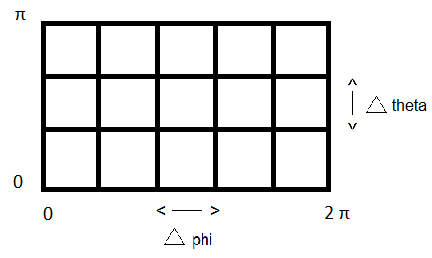
\includegraphics[scale=0.5]{Bilder/Gitter_phi_theta}
		\end{minipage}
		\hfill 
		\begin{minipage}{0.5\textwidth}
			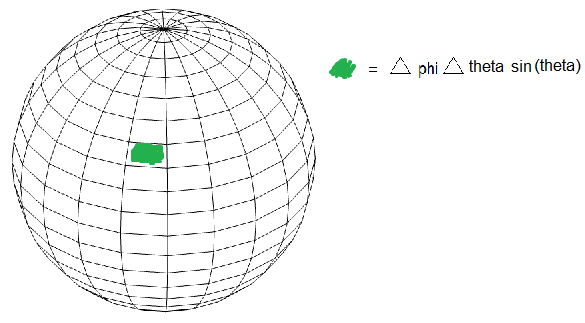
\includegraphics[scale=0.48]{Bilder/Kugel_mit_grid}
		\end{minipage}
	\caption{Grid on sphere}
	\end{figure}
\end{frame}



%%%%%%%%%%%%%%%%%%%%%%
% Properties
%%%%%%%%%%%%%%%%%%%%%%

\begin{frame}{Properties of harmonic polynomial basis functions}
	\begin{itemize}
		\item $\Delta_{S^2}P^i_n = -n(n+1) P^i_n$
		\vspace{12pt}
		\item $	f(\phi, \theta) = f_0 \cdot P_0^0 + \sum_{n=1}^{\infty} \sum_{i=-2n}^{2n} c^i_{2n} \cdot P^i_{2n}(\phi, \theta)$
		\vspace{12pt}
		\item $(P^i_n, P^l_m)_{S^2} = 0, \forall i \neq l \; \text{or} \; n \neq m$
		\vspace{12pt}
		\item $	(P^i_n, P^i_n)_{S^2} = 1$
	\end{itemize}
\end{frame}

\begin{frame}{Harmonic polynomial basis functions}
	\scriptsize
	Basis function ${P}^{i}_{n}(\phi, \theta)$, $n = 0, ..., \infty$ and $i = n, ..., -n$ are computed from orthogonal polynomials (Legendre polynomials). 
	\vspace{20pt}
	\begin{figure}
		\centering
		\subfloat[$P^0_0$]{
\includegraphics[width=2cm,height=2cm]{Bilder/P0_Kugel}}
		\qquad
		\subfloat[$P^{-1}_2$]{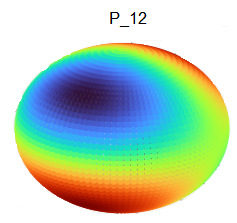
\includegraphics[width=2cm,height=2cm]{Bilder/P_12_Kugel}}
		\qquad
		\subfloat[$P^0_2$]{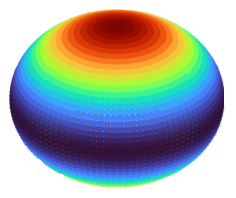
\includegraphics[width=2cm,height=2cm]{Bilder/P02_Kugel}}
		\qquad
		\subfloat[$P^{-1}_4$]{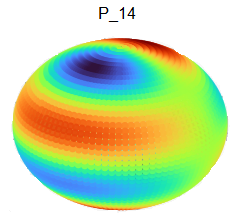
\includegraphics[width=2cm,height=2cm]{Bilder/P_14_Kugel}}
		\caption{Some harmonic polynomial basis functions}
	\end{figure}

	\begin{minipage}[b]{0.4\textwidth}
		\begin{table}[H]
			\tiny
			\begin{tabular}{|c|c|}
				\hline
				0th order & 2nd order \\
				\hline
				& $P^{-2}_2 = \sqrt{\frac{15}{16\pi}}\sin^2(\theta)\cos(2\phi)$ \\
				& $P^{-1}_2 = \sqrt{\frac{15}{4\pi}}\sin(\theta)\cos(\theta)\cos(\phi)$ \\
				$P^0_0 = \sqrt{\frac{1}{4\pi}} \cdot 1$ & $P^0_2 = \sqrt{\frac{45}{16\pi}}\cos^2(\theta) - \frac{1}{3}$ \\
				& $P^1_2 = \sqrt{\frac{15}{4\pi}}\sin(\theta)\cos(\theta)\sin(\phi)$\\
				& $P^2_2 = \sqrt{\frac{15}{16\pi}}\sin^2(\theta)\sin(2\phi)$\\
				\hline
			\end{tabular}
		\end{table}
	\end{minipage}
\end{frame}


\begin{comment}
\begin{frame}{Harmonic polynomial basis functions}
	\scriptsize
	Let ${P}^{i}_{n}(\phi, \theta)$ with $n = 0, ..., \infty$ and $i = n, ..., -n$ be the basis function
	\begin{align*}
		TODO
	\end{align*}
	The scalar product of any two basis functions over sphere is defined as follows
	\begin{align*}
		<P^i_n, P^l_m>_{S^2} = \int_{0}^{2\pi} \int_{0}^{\pi} P^{i}_{n}(\phi, \theta) \cdot P^{l}_{m}(\phi, \theta) \cdot \sin(\theta) d\theta d\phi.
	\end{align*}
\end{frame}
\end{comment}

\begin{comment}
\begin{frame}{Properties of harmonic polynomial basis functions}
	\scriptsize
	\begin{block}{Property 1}
		Let $P^{i}_{n}(\phi, \theta)$ and $P^{l}_{m}(\phi, \theta)$ are two different harmonic polynomial basis functions. Then
		\begin{align*}
			<P^i_n, P^l_m>_{S^2} = 0,
		\end{align*}
	for $i \neq l$ or $n \neq m$.
	\end{block}
	
	\begin{block}{Property 2}
		Let $P^i_{n}$ be the normalized harmonic polynomial basis functions. Then
		\begin{align*}
			<P^i_n, P^i_n>_{S^2} = 1.
		\end{align*}
	\end{block}

	\begin{block}{Property 3}
		The spherical harmonic function are the eigenfunctions of Laplace-Beltrami operator with the eigenvalues $(- n (n +1),n \in \mathbb{N}_0)$(see \cite{zbMATH01218597})
		\begin{align*}
			\Delta_{S^2}P^i_n = -n(n+1) P^i_n.
		\end{align*}
	\end{block}
\end{frame}
\end{comment}

%%%%%%%%%%%%%%%%%%%%%%%%%%%%%%%%%%%%%%
% Back to the spectral method
%%%%%%%%%%%%%%%%%%%%%%%%%%%%%%%%%%%%%%

\begin{frame}{Spectral method}
	\scriptsize
	Kinetic Smochluchowski equation on $S^2$:
	\begin{align}
		\underbrace{\sin \theta \partial_t f}_{[1]} + \underbrace{\partial_\phi\left(a(\phi, \theta) f\right)+\partial_\theta\left(b(\phi, \theta) f\right)}_{[2]} = \underbrace{D_r \left(\partial_\phi\left(\frac{1}{\sin \theta} \partial_\phi f\right)+\partial_\theta\left(\sin \theta \partial_\theta f\right)\right)}_{[3]} \label{Smoch_S2}
	\end{align}	
	Ansatz: $f(\phi, \theta, t) = f_0(t) \cdot P_0^0 + \sum_{n=1}^{N} \sum_{i=-2n}^{2n} c^i_{2n}(t) \cdot P^i_{2n}(\phi, \theta)$
 	\vspace{12pt}
 	\begin{itemize}
 		\item Insert ansatz for $f$ in (\ref{Smoch_S2}) 
 		\item Multiply consecutively with all basis functions used in the ansatz and integrate the resulting equations over $\phi$ and $\theta$
 	\end{itemize}
\end{frame}

\begin{frame}{Example}
	\scriptsize
	For  $f(\phi, \theta, t) = c^0_0(t) + \sum_{i=-2}^{2} c^i_{2}(t) \cdot P^i_{2}(\phi, \theta)$ we obtain
		\begin{equation}
		\left(\begin{array}{c}
			f_0(t) \\
			c_2^{-2}(t) \\
			c_2^{-1}(t) \\
			c_2^0(t) \\
			c_2^1(t) \\
			c_2^2(t)
		\end{array}\right)^{\prime} - A \cdot
		\left(\begin{array}{c}
			f_0(t) \\
			c_2^{-2}(t) \\
			c_2^{-1}(t) \\
			c_2^0(t) \\
			c_2^1(t) \\
			c_2^2(t)
		\end{array}\right) = -6 D_r \cdot
		\left(\begin{array}{c}
			0 \\
			c^{-2}_2(t) \\
			c_2^{-1}(t) \\
			c_2^0(t) \\
			c_2^1(t) \\
			c_2^2(t)
		\end{array}\right)
	\end{equation}
\end{frame}


%%%%%%%%%%%%%%


\begin{frame}
	For $N = 1$ the matrix $A$ has the form \\
	\vspace{20pt}
	\resizebox{\textwidth}{!}{
	\begin{equation*}
		\begin{pmatrix}
			\vspace{10pt}
			0 & 0 & 0 & 0 & 0 & 0 \\
			\vspace{12pt}
			\frac{1}{5}\sqrt{15}(u_x-v_y) & \frac{1}{7}(u_x+v_y-2w_z) & \frac{1}{7}(-5u_z+2w_x) & \frac{1}{7}\sqrt{3}(-u_x+v_y) & \frac{1}{7}(5v_z-2w_y) &  (u_y -v_x) \\
			\vspace{12pt}
			\frac{1}{5}\sqrt{15}(-u_z-w_x) & \frac{1}{7}(2u_z-5w_x) & \frac{1}{7}(u_x-2v_y+w_z) & \frac{1}{7}\sqrt{3}(-4u_z+3w_x) & \frac{1}{7}(5u_y-2v_x) &  \frac{1}{7} \left(2v_z-5w_y\right) \\
			\vspace{12pt}
			\frac{1}{5}\sqrt{5}(-u_x-v_y+2w_z) & \frac{1}{7}\sqrt{3}(-u_x+v_y) & \frac{1}{7}\sqrt{3}(3u_z-4w_x) & \frac{1}{7}(-u_x-v_y+2w_z) & \frac{1}{7}\sqrt{3}(-3v_z-4w_y) & \frac{1}{7} \sqrt{3}\left(-u_y-v_x\right) \\
			\vspace{12pt}
			\frac{1}{5}\sqrt{15}(-v_z-w_y) & \frac{1}{7}(-2v_z+5w_y) & \frac{1}{7}(-2u_y+5v_x) & \frac{1}{7}\sqrt{3}(-4v_z+3w_y) & \frac{1}{5}\sqrt{15}(-u_z-w_x) &  \frac{1}{7} \left(2u_z-5w_x\right)\\
			\vspace{12pt}
			\frac{1}{5}\sqrt{15}(u_y+v_x) & (-u_y+v_x) & \frac{1}{7}(-5v_z+2w_y) & \frac{1}{7}\sqrt{3}(-u_y-v_x) & \frac{1}{7}(-5u_z+2w_x) & \frac{1}{7} \left(u_x+v_y-2w_z\right)
		\end{pmatrix}
	\end{equation*}
	}
\end{frame}




\begin{comment}
\begin{frame}
	\scriptsize
	
	The Laplace Beltrami operator (\cite{zbMATH07295185}) on the unit sphere $S^2$ is given by
	\begin{align}
		\Delta_{S^2} f = \frac{1}{\sin ^2 \theta} \partial_{\phi \phi} f + \frac{1}{\sin \theta} \partial_\theta\left(\sin \theta \partial_\theta f\right). \label{laplace_eq}
	\end{align}
	From property 3 and the equation $(\ref{laplace_eq})$, it follows for the term (3)
	\begin{align*}
		\Delta_{S^2} P^i_{2n} = -n(n+1)P^i_{2n}.
	\end{align*}
	For the term $(1)$ and $(2)$, we inserting (5) in (4), multiplying with each basis function and integrate it over $S^2$. We derive a system of ODEs for the coefficients
	\scriptsize
	\begin{equation}
		\left(\begin{array}{c}
			f_0 \\
			c_2^{-2} \\
			\vdots \\
			c_{2n}^i
		\end{array}\right)^{\prime}=A\left(\begin{array}{c}
			f_0 \\
			c_2^{-2} \\
			\vdots \\
			c_{2n}^i
		\end{array}\right),
	\end{equation}
with $A \in \mathbb{R}^{cnxcn}$
\begin{equation*}
	c n= \begin{cases}\text { order }=2: & cn= 2 \cdot \text {order}+2 \\ \text { order }=\text {even: } & c2=6 \\  &c n=c2 \\ &c n=c2+\sum_{i=4}^{order}(2 i+1)\end{cases}
\end{equation*}
\end{frame}

%%%%%%%%%%%%%%%%%%
% Example
%%%%%%%%%%%%%%%%%%

\begin{frame}
	\centering
	Example: Shear flow
\end{frame}

\begin{frame}{Example: Shear flow}
	\scriptsize
	Consider the Smoluchowski equation $(\ref{Smoch_S2})$ with the velocity gradient 
	\begin{align*}
		\vec{u}=\left(\begin{array}{l}
			u(x,y,z) \\
			v(x,y,z) \\
			w(x,y,z)
		\end{array}\right),
		\nabla_x \vec{u}_{\mathrm{ext}}=\left(\begin{array}{lll}
			u_{x} & u_{y} & u_{z} \\
			v_{x} & v_{y} & v_{z} \\
			w_{x} & w_{y} & w_{z}
		\end{array}\right)=\left(\begin{array}{ccc}
			0 & 1 & 0 \\
			0 & 0 & 0 \\
			0 & 0 & 0
		\end{array}\right) .
	\end{align*}
	With the given velocity gradient it follows
	\begin{align}
		\partial_{t}\left(\sin \theta f\right) &+ \partial_\theta\left(\sin \phi \cos \phi \sin ^2 \theta \cos \theta f\right)+ \partial_\phi\left(- \sin \theta \sin ^2 \phi f \right) \nonumber \\
		&=D_{r}\left(\partial_\theta \left(\sin \theta \partial_\theta f\right)+ \partial_\phi\left(\frac{1}{\sin \theta} \partial_\phi f\right)\right). \label{smoEq} 
	\end{align}
	Consider the ansatz with the zeroth order
	\begin{align}
		f(\phi, \theta, t)= f_0(t) \cdot P_0^0 \label{ansatz_0nd}.
	\end{align}

	Insert the ansatz (\ref{ansatz_0nd}) in (\ref{smoEq})
	\begin{align}
		\partial_{t}(f_0(t) \cdot P_0^0)+\frac{1}{\sin \theta}\left(\partial_\theta(\ldots)+\partial_\phi(\ldots)\right)=\frac{1}{\sin \theta} D_r \left(\ldots \right) \label{eq_mitAnsatz}.
	\end{align}
\end{frame}

\begin{frame}
	\scriptsize
	We know
	\begin{align*}
		\Delta_{S^2} P_0^0(\phi, \theta) = \frac{1}{\sin \theta} D_r (\ldots) = \lambda_{2n,i} \cdot P^{0}_0(\phi, \theta),
	\end{align*}
	where $\lambda_{2n,i}$ is the corresponding eigenvalue.\\
	Since $P_0^0(\phi, \theta) = 1$ does not depend on $\phi$ and $\theta$, the partial derivatives will be zero
	\begin{align}
		\Delta_{S^2} P_0^0(\phi, \theta) = 0.
	\end{align}
	Consider the rest of the equation (\ref{eq_mitAnsatz})
	\begin{align*}
		\underbrace{\partial_{t}(f_0(t) \cdot P_0^0)}_{(1)}+ \underbrace{\frac{1}{\sin\theta}\left( \partial_\theta(\sin \phi \cos \phi \sin ^2 \theta \cos \theta \cdot f_0(t) \cdot P_0^0)+ \partial_\phi(- \sin \theta \sin ^2 \phi \cdot f_0(t) \cdot P_0^0)\right)}_{(2)}.
	\end{align*}
	It is
	\begin{align*}
		\partial_t\left(f_0(t) \cdot P^0_0\right)=f_0^{\prime}(t).
	\end{align*}
	Let $z(\phi, \theta) := (2)$
\end{frame}

\begin{frame}
	\scriptsize
	Project the solution $z(\phi, \theta)$ onto all polynomials to find out which polynomial are needed
	\begin{align*}
		\int_{0}^{2\pi} \int_{0}^{\pi} z(\phi, \theta) \cdot P^{-2}_2(\phi, \theta) \, \sin \theta d\theta d\phi &\overset{Maple}{=} 0 \\
		\int_{0}^{2\pi} \int_{0}^{\pi} z(\phi, \theta) \cdot P^{-1}_2(\phi, \theta) \, \sin \theta d\theta d\phi &\overset{Maple}{=} 0 \\
		\int_{0}^{2\pi} \int_{0}^{\pi} z(\phi, \theta) \cdot P^{0}_2(\phi, \theta) \, \sin \theta d\theta d\phi &\overset{Maple}{=} 0 \\
		\int_{0}^{2\pi} \int_{0}^{\pi} z(\phi, \theta) \cdot P^{1}_2(\phi, \theta) \, \sin \theta d\theta d\phi &\overset{Maple}{=} 0 \\
		\int_{0}^{2\pi} \int_{0}^{\pi} z(\phi, \theta) \cdot P^{2}_2(\phi, \theta) \, \sin \theta d\theta d\phi &\overset{Maple}{=} -\frac{\sqrt{15}}{5}
	\end{align*}
\end{frame}

\begin{frame}
	\scriptsize
	It follows
	\begin{align}
		f_0(t) \cdot P^0_0 \cdot \frac{1}{\sin \theta}\left(\partial_\theta\left(\sin \phi \cos \phi \sin ^2 \theta \cos \theta\right)+\partial_\phi \left(-\sin \theta \sin ^2 \phi\right)\right) = f_0(t) \left[ -\frac{\sqrt{15}}{2} P^2_2 \right]. \label{teil1}
	\end{align}
	Together we have
	\begin{align*}
		f_0^{\prime}(t)-\frac{\sqrt{15}}{2} f_0(t) P_2^2(\phi,\theta) = 0\cdot  P^0_0(\phi, \theta)  D_r.
	\end{align*}
\end{frame}

\begin{frame}
	\scriptsize
	\centering
	For the ansatzfunction with higher order, the calculation is done in the same way. \\
	As an example we obtain an ODE system with ansatzfunction of the $2nd.$ order
	\begin{equation}
		\left(\begin{array}{c}
			f_0^{\prime}(t) \\
			c_2^{-2} \\
			c_2^{-1} \\
			c_2^0 \\
			c_2^1 \\
			c_2^2
		\end{array}\right)=\left(\begin{array}{cccccc}
			0 & 0 & 0 & 0 & 0 & 0 \\
			0 & -6 D_r & 0 & 0 & 0 & 1 \\
			0 & 0 & -6 D_r & 0 & 5/7 & 0 \\
			0 & 0 & 0 & -6 D_r & 0 & -\frac{\sqrt{3}}{7} \\
			0 & 0 & -2/7 & 0 & -6 D_r & 0 \\
			\frac{\sqrt{15}}{5} & 1 & 0 & -\frac{\sqrt{3}}{7} & 0 & -6 D_r
		\end{array}\right) \cdot\left(\begin{array}{c}
			f_0 \\
			c_2^{-2} \\
			c_2^{-1} \\
			c_2^0 \\
			c_2^1 \\
			c_2^2
		\end{array}\right)
	\end{equation}
\end{frame}

\begin{frame}
	\begin{table}[H]
		\scriptsize
		\begin{tabular}{|c|c|}
			\hline
			0th order	& 2nd order \\
			\hline
			& $P^{-2}_2 = \sqrt{\frac{15}{16\pi}}\sin^2(\theta)\cos(2\phi)$ \\
			& $P^{-1}_2 = \sqrt{\frac{15}{4\pi}}\sin(\theta)\cos(\theta)\cos(\phi)$ \\
			$P^0_0 = \sqrt{\frac{1}{4\pi}} \cdot 1$	& $P^0_2 = \sqrt{\frac{45}{16\pi}}\cos^2(\theta) - \frac{1}{3}$  \\
			&  $P^1_2 = \sqrt{\frac{15}{4\pi}}\sin(\theta)\cos(\theta)\sin(\phi)$\\
			&  $P^2_2 = \sqrt{\frac{15}{16\pi}}\sin^2(\theta)\sin(2\phi)$\\
			\hline
		\end{tabular}
		\caption{Normalized harmonic polynomial basis functions.}
	\end{table}
\end{frame}
\end{comment}

%\begin{frame}
%	\begin{itemize}
%		\item The harmonic polynomial basis function of the second order are the eigenfunctions of the Laplace Beltrami operator with eigenvalue $-6$. 
%		\item $P^{-4}_4, ..., P^4_4$ are eigenfunctions of the Laplace Beltrami operator with eigenvalue $-20$.
		%\item For higher order there exist also an eigenvalue relation the Laplace Beltrami operator.
%	\end{itemize}
%\end{frame}


